%Autor: Simon Walker
%Version: 1.0
%Datum: 10.11.2019

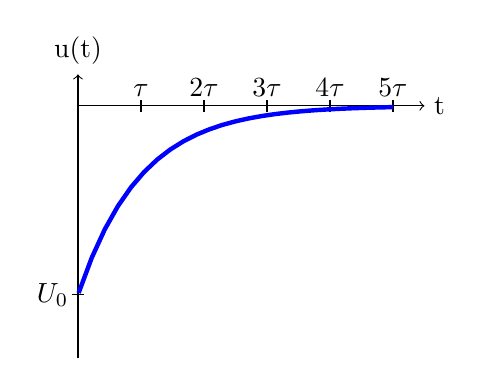
\begin{tikzpicture}[xscale=0.8, yscale=0.8]
	%\draw[help lines] (0,0) grid (6,4);
	\normalsize
	\draw [->] (0, 4) -- (0, 4.5);
	\draw [<-] (5.5, 4) --  (0, 4) -- (0, 0);
	\node [right] at (5.5, 4) {t};
	\node [above] at (0, 4.5) {u(t)};
	
	\draw (1, 3.9) --  (1, 4.1);
	\node [above] at (1, 4) {$\tau$};
	\draw (2, 3.9) --  (2, 4.1);
	\node [above] at (2, 4) {$2\tau$};
	\draw (3, 3.9) --  (3, 4.1);
	\node [above] at (3, 4) {$3\tau$};
	\draw (4, 3.9) --  (4, 4.1);
	\node [above] at (4, 4) {$4\tau$};
	\draw (5, 3.9) --  (5, 4.1);
	\node [above] at (5, 4) {$5\tau$};
	
	
	\node [left] at (0, 1) {$U_0$};
	\draw (-0.1, 1) --  (0.1, 1);
	\draw[blue, ultra thick, domain=0.01:5] plot (\x, {(-3)*e^(-\x) + 4});
\end{tikzpicture}
